\documentclass[a4 paper]{article}
% Set target color model to RGB
\usepackage[inner=2.0cm,outer=2.0cm,top=2.5cm,bottom=2.5cm]{geometry}
\usepackage{setspace}
\usepackage[rgb]{xcolor}
\usepackage{verbatim}
\usepackage{subcaption}
\usepackage{amsgen,amsmath,amstext,amsbsy,amsopn,tikz,amssymb,tkz-linknodes}
\usepackage{fancyhdr}
\usepackage[colorlinks=true, urlcolor=blue,  linkcolor=blue, citecolor=blue]{hyperref}
\usepackage[colorinlistoftodos]{todonotes}
\usepackage{rotating}
\usepackage{float}

\usepackage{booktabs}
\newcommand{\ra}[1]{\renewcommand{\arraystretch}{#1}}

\newtheorem{thm}{Theorem}[section]
\newtheorem{prop}[thm]{Proposition}
\newtheorem{lem}[thm]{Lemma}
\newtheorem{cor}[thm]{Corollary}
\newtheorem{defn}[thm]{Definition}
\newtheorem{rem}[thm]{Remark}
\numberwithin{equation}{section}

\newcommand{\homework}[6]{
   \pagestyle{myheadings}
   \thispagestyle{plain}
   \newpage
   \setcounter{page}{1}
   \noindent
   \begin{center}
   \framebox{
      \vbox{\vspace{2mm}
    \hbox to 6.28in { {\bf COL774:~Machine Learning \hfill { #2}} }
       \vspace{6mm}
       \hbox to 6.28in { {\LARGE \hfill #1  \hfill} }
       \vspace{6mm}
       \hbox to 6.28in {\bf {Entry Number: {\rm #4} \hfill Name: {\rm #5} } }
       % \hbox to 6.28in { {\it TA: #4  \hfill #6}}
      \vspace{2mm}}
   }
   \end{center}
   \markboth{#1}{#1}
   \vspace*{4mm}
}

% \newcommand{\problem}[2]{~\\\fbox{\textbf{Problem #1}}\hfill (#2 points)\newline\newline}
% \newcommand{\subproblem}[1]{~\newline\textbf{(#1)}}
% \newcommand{\D}{\mathcal{D}}
% \newcommand{\Hy}{\mathcal{H}}
% \newcommand{\VS}{\textrm{VS}}
% \newcommand{\solution}{~\newline\textbf{\textit{(Solution)}} }

% \newcommand{\bbF}{\mathbb{F}}
% \newcommand{\bbX}{\mathbb{X}}
% \newcommand{\bI}{\mathbf{I}}
% \newcommand{\bX}{\mathbf{X}}
% \newcommand{\bY}{\mathbf{Y}}
% \newcommand{\bepsilon}{\boldsymbol{\epsilon}}
% \newcommand{\balpha}{\boldsymbol{\alpha}}
% \newcommand{\bbeta}{\boldsymbol{\beta}}
% \newcommand{\0}{\mathbf{0}}

\begin{document}
\homework{Assignment 2 Report}{Date: March 15, 2019}{}{\bf 2016CS10363}{\bf Manish Tanwar}{NetId(s)}

\vspace*{-4mm}
\section{Naive Bayes:}
\subsection*{(a) Accuracy over test and training dataset:}
	\begin{itemize}
	\item Accuracy over test dataset: \textbf{60.4 \%}
	\item Accuracy over training dataset: \textbf{64.6 \%}
	\end{itemize}

\subsection*{(b) Accuracy using Random and Majority Prediction:}
	\begin{itemize}
	\item Accuracy using Random Prediction: \textbf{19.9 \%}
	\item Accuracy using Majority Prediction: \textbf{44.0 \%}
	\end{itemize}

\subsection*{(c) Confusion Matrix:}
	\begin{figure}[ht!]
		\centering %width=90mm
		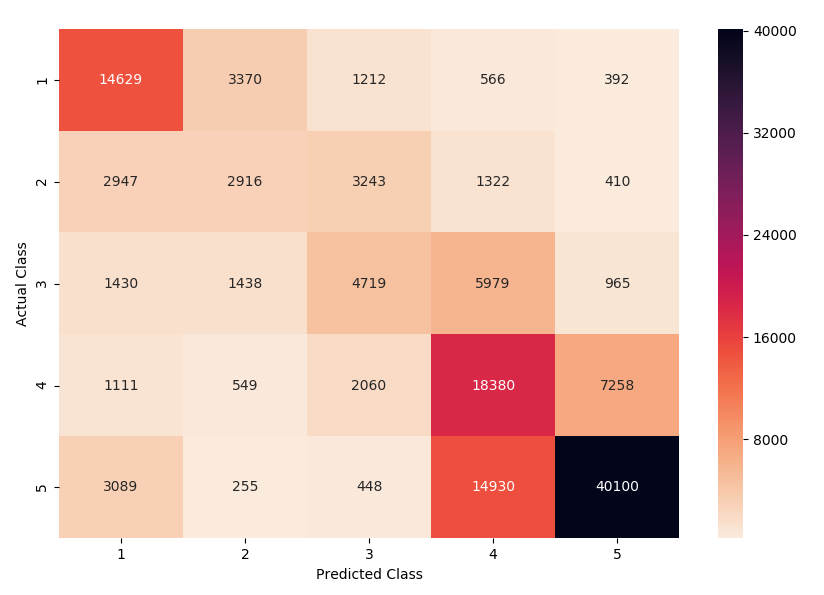
\includegraphics[width=150mm]{extra/1c.png}
		\caption{Confusion Matrix\label{MIMD}}
	\end{figure}

	\begin{itemize}
	\item Diagonal has the most elements which represents the correct predictions.
	\item Confusion matrix also shows the correlation between adjacent ratings.(For example for actual class 5, it has most entries in 5 but it has second most entries in 4).
	\item The number of elements decreases as we move away from the diagonal which shows clear correlation.
	\end{itemize}

\subsection*{(d) Stemming and Stopword Removal:}
	\begin{itemize}
	\item Accuracy Obtained: \textbf{60.0 \%}
	\item Accuracy does not change much on performing stemming and stopword removal.
	\end{itemize}

\subsection*{(e) Feature Engineering:}
	\begin{itemize}
	\item Accuracy Obtained: \textbf{63.4 \%}
	\item On adding bigram feature on top of our model, accuracy increases by \textbf{3-4\%}.
	\item Using bigrams feature introduces dependencies among words which increases the accuracy.
	\end{itemize}

\subsection*{(f) F1-Score:}
	% F1_score: [0.7193 0.2362 0.2805 0.5231 0.7821]
	% 	macro_f1_score: 0.5083061917191372
	\begin{itemize}
	\item F1 Score : $ [0.7193 \quad 0.2362 \quad 0.2805 \quad 0.5231 \quad 0.7821] $
	\item Less F1 score for class 2 and 3 shows less accuracy for these classes.
	\item Macro F1 Score : \textbf{0.5083}
	\item Macro F1 score is a better metric, especially in uneven class distribution model as it considers both precision and recall to compute the score.
	\end{itemize}

\subsection*{(g) Training of Full Dataset:}
	\begin{itemize}
	\item Accuracy Obtained: \textbf{73.15\%}
	\item F1 Score : $ [0.7645 \quad 0.5130 \quad 0.5901 \quad 0.6533 \quad 0.8336] $
	\item Macro F1 Score : \textbf{0.6709}
	\item Increase in training data helps in better model learning and prediction.
	\end{itemize}

\section{Support Vector Machine:}
\subsection{Binary Classification:}
\vspace*{4mm}
\subsection*{(a) CVXOPT with Linear Kernel:}
	\begin{itemize}
	\item Accuracy Obtained: \textbf{99.49\%}
	\item Indices of Support Vectors, Weights($w$) and bias($b$) are submitted in file \text{"linear\_results.txt"}
	\item Number of Support Vectors: 134
	\end{itemize}

\subsection*{(b) CVXOPT with Gaussian Kernel:}
	\begin{itemize}
	\item Accuracy Obtained: \textbf{99.89\%}
	\item Indices of Support Vectors are submitted in file \text{"gaussian\_results.txt"}
	\item Number of Support Vectors: 1386
	\end{itemize}

\subsection*{(c) LIBSVM Package with Linear and Gaussian Kernels:}
	\subsubsection*{\hspace*{3mm}Linear Kernel:}
	\begin{itemize}
	\item Accuracy Obtained: \textbf{99.49\%}
	\item Indices of Support Vectors, Weights($w$) and bias($b$) are submitted in file \text{"libsvm\_linear\_results.txt"}
	\item Number of Support Vectors: 134
	\end{itemize}
	
	\subsubsection*{\hspace*{3mm}Gaussian Kernel:}
	\begin{itemize}
	\item Accuracy Obtained: \textbf{99.89\%}
	\item Indices of Support Vectors are submitted in file \text{"libsvm\_gaussian\_results.txt"}
	\item Number of Support Vectors: 1344
	\end{itemize}

\subsubsection*{\hspace*{3mm}Computational Cost Comparision:}
\hskip4.0cm\begin{tabular}{ |p{2cm}||p{2cm}|p{2cm}|}
	 \hline
	 \multicolumn{3}{|c|}{Training Time(in Sec)} \\
	 \hline Kernel & CVXOPT & LIBSVM\\
	 \hline
	 Linear & 74.82 & 4.59\\
	 Gaussian & 35.84 & 8.96\\
	 \hline
\end{tabular}

\begin{itemize}
\item LIBSVM takes way less time than CVXOPT package.
\item Using CVXOPT and LIBSVM gives almost same \textbf{number of support vectors}. Slight difference is due to floating point arithmetic comparison $ \alpha > 0 $, which is done using $ \alpha > eps \quad (eps = 10^{-5}) $.
\end{itemize}


\subsection{Multi-Class Classification:}
\vspace*{4mm}
\subsection*{(a) Using CVXOPT Package:}
	\begin{itemize}
	\item Accuracy over test dataset: \textbf{97.24 \%}
	\item Accuracy over training dataset: \textbf{99.92 \%}
	\end{itemize}

\subsection*{(b) Using LIBSVM Package:}
	\begin{itemize}
	\item Accuracy over test dataset: \textbf{97.23 \%}
	\item Accuracy over training dataset: \textbf{99.92 \%}
	\end{itemize}

% \subsubsection*{\hspace*{3mm}Computational Cost Comparision:}
\textbf{Computational Cost Comparision }(Training time):
\begin{itemize}
\item CVXOPT : 472.36 sec
\item LIBSVM : 237.51 sec
\end{itemize}

\subsection*{(c) Confusion Matrix:}

	\begin{figure}[H]
		\centering %width=90mm
		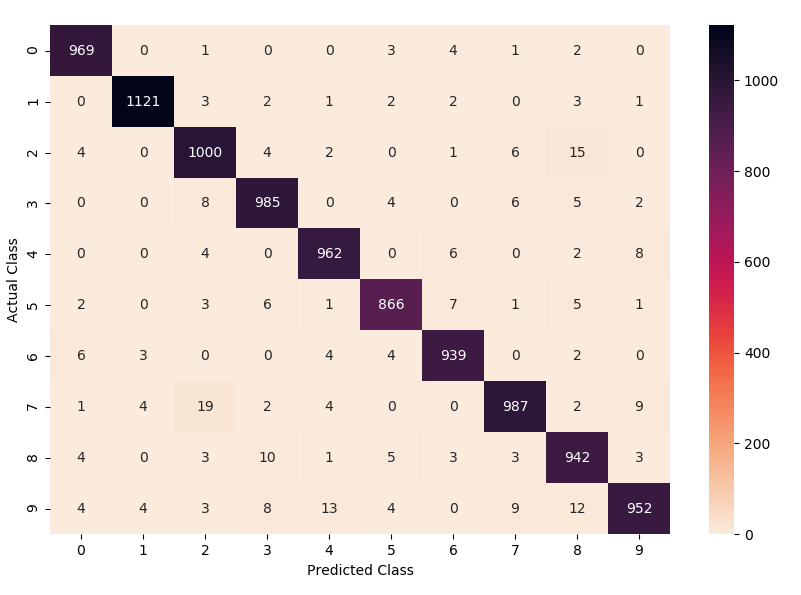
\includegraphics[width=150mm]{extra/2c.png}
		\caption{Confusion Matrix(drawn for part(b))\label{MIMD}}
	\end{figure}

	\textbf{Analysis:}
	\begin{itemize}
	\item Most often 2,7,8,9 are misclassified as 8,2,3,4 respectively.
	\item Misclassification of 7 as 2, 8 as 3 and 9 as 4 is due to their similarity in structural representation.
	\end{itemize}

\subsection*{(d) Validation:}
	
	\begin{itemize}
		\item We randomly select 10\% data from trainig dataset as validation set to estimate the parameter $C$.
		\item $C$ is penalty parameter. Value of parameter $C$ how much misclassification do we allow for finding the hyperplane.
		\item For $C = 5 \text{ and } 10$, we obtain the best validation and test accuracy.
		\item For smaller $C$, we allow too much misclassification by imposing too low penalty which results in really low accuracy.
	\end{itemize}

	\hskip4.0cm\begin{tabular}{ |p{1cm}||p{2cm}|p{2cm}|}
	 % \hline
	 % \multicolumn{3}{|c|}{Training Time(in Sec)} \\
	 \hline $C$ & Validation Accuracy & Test Accuracy\\
	 \hline
	 	$10^{-5}$	&9	& 10.28\\
		$10^{-3}$	&9	& 10.28\\
		1		&97.7	& 97.12\\
		5		&97.8	& 97.24\\
		10		&97.8	& 97.24\\
	 \hline
	\end{tabular}

	\begin{figure}[H]
		\centering %width=90mm
		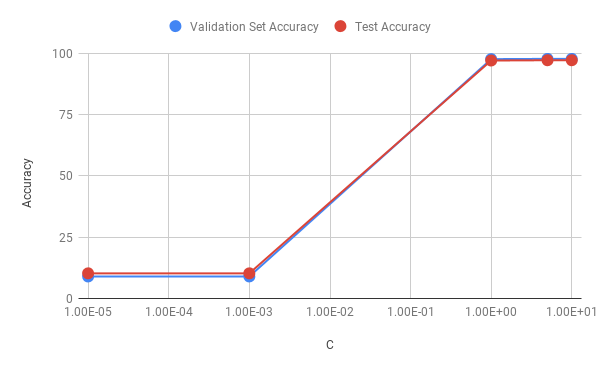
\includegraphics[width=150mm]{extra/chart.png}
		\caption{Accuracy Vs Parameter $C$\label{MIMD}}
	\end{figure}

\end{document}